% 隔離テスト用ドライバ: 9-12 のみを単独ビルド（共有 main.tex には影響しない）
\documentclass[11pt,aspectratio=43,dvipsnames]{beamer}
\usepackage{luatexja}
\usepackage[match]{luatexja-fontspec}
\setmainjfont{HaranoAjiGothic}
\setsansjfont{HaranoAjiGothic}
\renewcommand{\kanjifamilydefault}{\gtdefault}
\usepackage{amsmath, amssymb}
\usepackage[version=4]{mhchem}
\usepackage{booktabs}
\usepackage{multirow}
\usepackage{colortbl}
\usepackage{graphicx}
\graphicspath{{figures/}}
% =====================================================================
%  seminar テーマ定義（既存 Marp デザインの Beamer 再現）
%  ・濃青の恒常ヘッダーバー（セクション名＋ページ番号）
%  ・専用表紙（アクセントライン＋グラデ背景）
%  ・本文は白地・濃青見出し
%  main.tex から \input する（パッケージではなく生プリアンブル）
% =====================================================================

% ---- ベース：装飾の少ないテーマから組む -----------------------------
\usetheme{default}
\usefonttheme{professionalfonts}
\setbeamertemplate{navigation symbols}{}   % ナビゲーション記号を消す

% ---- TikZ（ヘッダー・表紙・矢印などで使用）-------------------------
\usepackage{tikz}
\usetikzlibrary{arrows.meta, positioning, calc, shapes.geometric, fit, patterns}

% ---- 配色（ルール準拠）---------------------------------------------
\definecolor{HeaderBlue}{HTML}{0f5a7a}   % ヘッダー・見出しの濃青
\definecolor{DateGray}{HTML}{334b5e}     % 表紙の日付グレー
\definecolor{TitleBG}{HTML}{edf5fb}      % 表紙グラデの薄青

% コンテンツ用パレット（図・ハイライト・矢印で共通利用）
\definecolor{ArrowBlue}{HTML}{1F6FC4}    % 矢印・強調の青
\definecolor{HiPink}{HTML}{F4B6BE}       % ハイライト見出し（暖色）
\definecolor{HiBlue}{HTML}{C7DCEF}       % ハイライト見出し（寒色）
\definecolor{IpaBlue}{HTML}{1F5FC4}      % グラフ系列1（青）
\definecolor{DipeOrange}{HTML}{E8821E}   % グラフ系列2（橙）
\definecolor{SpRed}{HTML}{C0392B}        % 反応式：プロピレン強調の赤
\definecolor{SpBlue}{HTML}{1F6FC4}       % 反応式：エテン・エタン・CH0.5 の青

% 帯（ヘッダーバー）のパート別配色（寒色グラデ）。本文枠線は HeaderBlue のまま。
%  1-4 導入・全体像／5-9 反応・反応器／10-13 分離／14-17 最適化・経済・結言
\definecolor{barA}{HTML}{0F5A7A}   % 1-4  青緑
\definecolor{barB}{HTML}{1D6E6E}   % 5-9  シアン寄り
\definecolor{barC}{HTML}{2E4C8A}   % 10-13 青
\definecolor{barD}{HTML}{4A3C84}   % 14-17 紫

\setbeamercolor{normal text}{fg=black, bg=white}
\setbeamercolor{frametitle}{fg=HeaderBlue, bg=white}
\setbeamercolor{itemize item}{fg=HeaderBlue}
\setbeamercolor{itemize subitem}{fg=HeaderBlue}
\setbeamercolor{block title}{fg=white, bg=HeaderBlue}
\setbeamercolor{block body}{fg=black, bg=TitleBG}
\setbeamercolor{alerted text}{fg=HeaderBlue}

% ---- フォントサイズ（Marp px をおおよそ pt に対応）------------------
\setbeamerfont{frametitle}{size=\large, series=\bfseries}   % スライド見出し ~44px

% ---- 恒常ヘッダーバー（headline）-----------------------------------
%  左：セクション名（無ければロゴ枠）／右：ページ番号
\newcommand{\HeaderLogo}{}   % ロゴを入れるなら \renewcommand で画像指定
% 本線の総枚数（分母）。appendix に入ると分子がこれを超え、本線/付録を見分けられる。
\newcommand{\MainTotal}{17}
% パート別に帯色を選ぶ：1-4=barA／5-9=barB／10-13=barC／14-17=barD。
% スライド4の独自帯（CC・GCC）など headline を上書きする箇所でも呼べるよう独立コマンド化。
% 併せて本文アクセント色 HeaderBlue 自体をそのパート色へ再定義し、各スライドの
% 図・枠線・矢印・ボックス（HeaderBlue 参照）をパート色に連動させる（\colorlet は大域的）。
% headline はフレーム本文より前に組まれるため、ここでの再定義が本文に効く。
\newcommand{\SetBarColor}{%
  \ifnum\insertframenumber<5\setbeamercolor{headerbar}{fg=white, bg=barA}\colorlet{HeaderBlue}{barA}%
  \else\ifnum\insertframenumber<10\setbeamercolor{headerbar}{fg=white, bg=barB}\colorlet{HeaderBlue}{barB}%
  \else\ifnum\insertframenumber<14\setbeamercolor{headerbar}{fg=white, bg=barC}\colorlet{HeaderBlue}{barC}%
  \else\setbeamercolor{headerbar}{fg=white, bg=barD}\colorlet{HeaderBlue}{barD}%
  \fi\fi\fi}
\setbeamertemplate{headline}{%
  \ifnum\insertframenumber>0\relax
    \SetBarColor
    \begin{beamercolorbox}[wd=\paperwidth, ht=4.5ex, dp=1.8ex,
                           leftskip=1.2em, rightskip=1.2em]{headerbar}%
      \color{white}\bfseries\large
      \insertsectionhead%
      \hfill
      \insertframenumber/\MainTotal%
    \end{beamercolorbox}%
  \fi
}
\setbeamercolor{headerbar}{fg=white, bg=barA}
\setbeamertemplate{footline}{}             % フッターは使わない
\setbeamersize{text margin left=3mm, text margin right=3mm}  % 本文を横幅ぎりぎりまで

% 【必須ルール】帯と本文の間の余白を詰める（全スライド共通）。
%  beamer 既定の天井スキップで本文が帯から離れるのを、headline 直後の負スキップで打ち消す。
%  情報量最優先：無駄な上余白は作らない。各スライドは [t] 推奨。
\addtobeamertemplate{headline}{}{\vskip-2.6ex}

% frametitle はバーの直下に置く（左寄せ・濃青・太字）
\setbeamertemplate{frametitle}{%
  \vskip0.6ex
  \hspace{0.6em}\usebeamerfont{frametitle}\usebeamercolor[fg]{frametitle}\insertframetitle\par
  \vskip0.2ex
}

% ---- 箇条書きをシンプルに ------------------------------------------
\setbeamertemplate{itemize item}{\textbullet}
\setbeamertemplate{itemize subitem}{--}

% =====================================================================
%  再利用ヘルパー（どのスライドでも使える共通部品）
% =====================================================================
% 青い矢印 →（行中に置ける。結論や対応関係の明示に）
\newcommand{\bluearrow}{\tikz[baseline=-0.5ex]\draw[ArrowBlue, line width=1pt,
  -{Stealth[length=2.2mm]}] (0,0)--(0.55,0);}

% ハイライト見出し  \hilite{色}{テキスト}  例: \hilite{HiPink}{IPA選択率の温度依存性}
\newcommand{\hilite}[2]{\colorbox{#1}{\bfseries\normalsize #2}}

% パラメータ表  \paramtable{ 項目 & 値 \\ ... }  （左:項目 右:値、単位は数式推奨）
\newcommand{\paramtable}[1]{%
  {\footnotesize\renewcommand{\arraystretch}{1.15}%
   \begin{tabular}{@{\hspace{1em}}ll@{}}#1\end{tabular}}}

% =====================================================================
%  専用表紙コマンド  \seminartitlepage
%  ルール準拠：アクセントライン(120x8px相当) + 160度グラデ背景
%               h1 60px / h2 34px濃青 / 著者27px / 日付22pxグレー
%  使い方: \title{} \subtitle{} \author{} \date{} を設定後に呼ぶ
% =====================================================================
\newcommand{\seminartitlepage}{%
  \begin{frame}[plain]
    \begin{tikzpicture}[remember picture, overlay]
      % 背景グラデ（左上 薄青 → 右下 白、斜め）
      \shade[top color=TitleBG, bottom color=white, shading angle=20]
        (current page.south west) rectangle (current page.north east);
      % アクセントライン（上から少し下げて左に）
      \fill[HeaderBlue]
        ([xshift=9mm, yshift=-12mm]current page.north west)
        rectangle ++(16mm, 1.1mm);
      % テキストブロック（左寄せ・縦中央付近）
      \node[anchor=center, text width=0.86\paperwidth, align=center]
            at (current page.center) {%
        {\fontsize{22pt}{28pt}\selectfont\bfseries\color{black}\inserttitle\par}
        \vspace{0.3em}
        {\fontsize{16pt}{20pt}\selectfont\bfseries\color{HeaderBlue}\insertsubtitle\par}
        \vspace{1.0em}
        {\fontsize{13pt}{17pt}\selectfont\color{black}\insertauthor\par}
        \vspace{0.4em}
        {\fontsize{11pt}{14pt}\selectfont\color{DateGray}\insertdate\par}
      };
    \end{tikzpicture}
  \end{frame}
}

\setlength{\overfullrule}{6pt}
\begin{document}
\setcounter{framenumber}{8}
\section{分離戦略}% =====================================================================
%  09  分離工程 — 反応器の前後で分けた整然ブロック図（一目で分かる）
%  source_memo: 05/06/07/08 章＋trial #201。前=脱ブタンでC4除去、
%   後=脱エタン→塔頂PSA(H2 99.9mol%)・塔底膜→C3塔(C3H6 99.5wt%)。
%   膜=最難 α≈1.07 を赤。製品を強調・副生/リサイクルは淡色。直交配線のみ。
%  方針：文章なし・斜め線なし・重なりなし。PFD(slide02)とは別物。
% =====================================================================
\begin{frame}

  \centering
  \resizebox{0.96\linewidth}{!}{%
  \begin{tikzpicture}[
    >=Stealth, font=\footnotesize,
    box/.style={draw=HeaderBlue, fill=HiBlue!45, rounded corners=2pt, align=center,
                inner sep=2pt, minimum width=16mm, minimum height=10mm},
    hard/.style={draw=SpRed, fill=SpRed!12, rounded corners=2pt, align=center,
                 inner sep=2pt, minimum width=16mm, minimum height=10mm},
    prod/.style={align=center, font=\footnotesize\bfseries},
    feed/.style={align=center, font=\footnotesize},
    side/.style={align=center, font=\scriptsize, text=black!55},
    ttl/.style={anchor=west, font=\bfseries},
    a/.style={-{Stealth[length=2mm]}, line width=0.9pt},
    g/.style={-{Stealth[length=1.8mm]}, line width=0.7pt, black!55},
    lab/.style={font=\scriptsize, fill=white, inner sep=1pt},
  ]
    % =================== 反応器の前 ===================
    \node[ttl] at (-0.6,3.0) {反応器の前};
    \node[feed] (fresh)  at (0,2.0)   {原料 LPG};
    \node[box]  (deb)    at (2.6,2.0) {脱ブタン塔\\{\tiny 蒸留}};
    \node[feed] (toreac) at (5.4,2.0) {反応器へ};
    \node[side] (c4)     at (2.6,0.85){$\mathrm{C_4}$ 留分 $\to$ 燃料};
    \draw[a] (fresh) -- (deb);
    \draw[a] (deb) -- (toreac);
    \draw[g] (deb.south) -- (c4.north);

    % 仕切り
    \draw[black!22, line width=0.5pt] (-1.0,0.25) -- (12.4,0.25);

    % =================== 反応器の後 ===================
    \node[ttl] at (-0.6,-0.4) {反応器の後};
    \node[feed] (rxout) at (0,-1.7)   {反応器\\出口ガス};
    \node[box]  (deeth) at (2.6,-1.7) {脱エタン塔\\{\tiny 蒸留}};
    % 上：塔頂→PSA→水素
    \node[box]  (psa)   at (6.0,-0.7) {PSA\\{\tiny 吸着}};
    \node[prod] (h2)    at (9.2,-0.35){$\mathrm{H_2}$ 製品\\{\scriptsize $99.9$ mol\%}};
    \node[side] (off)   at (9.2,-1.25){オフガス $\to$ 燃料};
    % 下：塔底→膜→C3塔→プロピレン
    \node[hard] (mem)   at (6.0,-2.7) {膜分離器\\{\tiny 膜}};
    \node[box]  (c3)    at (9.0,-2.7) {C3 スプリッタ\\{\tiny 蒸留}};
    \node[prod] (prod)  at (11.9,-2.7){$\mathrm{C_3H_6}$ 製品\\{\scriptsize $99.5$ wt\%}};
    \node[side] (rec)   at (9.0,-3.9) {未反応 $\mathrm{C_3H_8}$ $\to$ リサイクル};
    % 配線（直交のみ）
    \draw[a] (rxout) -- (deeth);
    \coordinate (split) at (4.3,-1.7);
    \draw[line width=0.9pt] (deeth.east) -- (split);
    \draw[a] (split) |- node[lab,pos=0.75]{軽質ガス} (psa.west);
    \draw[a] (split) |- node[lab,pos=0.75]{$\mathrm{C_3}$} (mem.west);
    \coordinate (psplit) at (7.7,-0.7);
    \draw[line width=0.9pt] (psa.east) -- (psplit);
    \draw[a] (psplit) |- (h2.west);
    \draw[g] (psplit) |- (off.west);
    \draw[a] (mem) -- node[lab]{$98.6$\%} (c3);
    \draw[a] (c3) -- (prod);
    \draw[g] (c3.south) -- (rec.north);
    \node[side, text=SpRed!80!black] at (6.0,-3.55) {最難 $\alpha\!\approx\!1.07$};
  \end{tikzpicture}}

\end{frame}

\section{蒸留分離}% =====================================================================
%  10  蒸留3塔まとめ — 共通モデルで設計、難易度は比揮発度で決まる
%  source_memo: 05/06/07 章＋最適化表 trial #201・検証出力。
%   脱ブタン P19.5/N36/H33/全凝縮/SM、脱エタン P7.9/N61/H52/部分凝縮/HYSYS、
%   C3スプリッタ P16.7/N117/H94/全凝縮/SM。α: 大 / ~3.9 / ~1.07。
%  方針：型G総覧。全幅比較表＋共通モデル注記。C3 の α・段数を注目色（赤）で。
%        蒸留単独では C3 が非現実→膜へ（次スライド）の伏線。丸括弧禁止。
% =====================================================================
\begin{frame}

  {\bfseries\large 共通モデルで3塔を設計、難易度は比揮発度 $\alpha$ で決まる}\par
  \vspace{0.15em}
  {\footnotesize 塔径はフラッディング許容蒸気速度、塔高は段効率 $0.8$、設備費は Bare Module 法で共通に評価する。}\par

  \vspace{0.7em}

  \centering
  {\footnotesize\renewcommand{\arraystretch}{1.22}%
   \begin{tabular}{@{}l c c c@{}}
     \toprule
      & 脱ブタン塔 & 脱エタン塔 & C3 スプリッタ \\
     \midrule
     役割          & 原料 $\mathrm{C_4}$ 除去 & 軽質ガス分離 & プロピレン精製 \\
     軽キー／重キー & $\mathrm{C_3H_8}/\mathrm{C_4H_{10}}$ & $\mathrm{C_2H_6}/\mathrm{C_3H_8}$ & $\mathrm{C_3H_6}/\mathrm{C_3H_8}$ \\
     比揮発度 $\alpha$ & 大 & $\approx 3.9$ & {\boldmath\color{SpRed}$\approx 1.07$} \\
     操作圧力      & $19.5$ bar & $7.9$ bar & $16.7$ bar \\
     理論段数      & $36$ & $61$ & {\boldmath\color{SpRed}$117$} \\
     塔高          & $33$ m & $52$ m & {\boldmath\color{SpRed}$94$ m} \\
     凝縮器        & 全凝縮 & 部分凝縮 & 全凝縮 \\
     評価モデル    & SM & HYSYS & SM \\
     \bottomrule
   \end{tabular}}\par

  \vspace{0.45em}

  \raggedright
  {\footnotesize
   \textbf{脱エタン塔}　$\mathrm{H_2},\mathrm{CH_4}$ が非凝縮のため部分凝縮で気相留分とし、塔頂 $-82\,^\circ$C の低温で軽質ガスを分離。非凝縮成分でサロゲート化が難しく HYSYS で直接評価\par
   \vspace{0.3em}
   \textbf{C3 スプリッタ}　$\alpha\!\approx\!1.07$ で段数 $117$・塔高 $94$ m と突出し装置設備費の過半を占める。$N_{\min}\!\propto\!1/\ln\alpha$ より\textbf{蒸留単独では非現実}\par
   \vspace{0.2em}
   \hspace{1.2em}$\to$\,\textbf{最難の $\mathrm{C_3H_6}/\mathrm{C_3H_8}$ 分離は膜と組み合わせて解く}}

\end{frame}

\section{プロピレン精製}% =====================================================================
%  11  プロピレン精製 — 膜×C3スプリッタ ハイブリッド（★主役・型F＋型G）
%  source_memo: 07_product_purification.tex（膜の定量的妥当性 Case A/B、
%   ZIF-8 MMM α=90・A_mem=1.28e5 m²・stage_cut 25%・透過98.6%、C3塔117段94m）。
%   図 membrane_vs_dist3.png（対数軸、膜なしは合計TAC 12倍・C3塔CAPEX 16.8倍）。
%  方針：左=証拠（膜有無の比較図＋数値）、右=採用ハイブリッド構成＋諸元。
%        アサーション＝難分離を物理原理の違う膜で解く。丸括弧禁止・色最小。
% =====================================================================
\begin{frame}

  {\bfseries\large $\alpha\!\approx\!1.07$ の最難分離は物理原理の違う膜で解く}\par
  \vspace{0.15em}
  {\footnotesize $\mathrm{C_3H_6}/\mathrm{C_3H_8}$ は沸点差 $6$ K で蒸留単独は $200$ 段・塔高 $156$ m と非現実。膜で粗濃縮し蒸留で仕上げる。}\par

  \vspace{0.2em}

  \begin{columns}[T,onlytextwidth]
    % ===== 左：膜有無の比較（証拠）================================
    \begin{column}{0.5\textwidth}
      \centering
      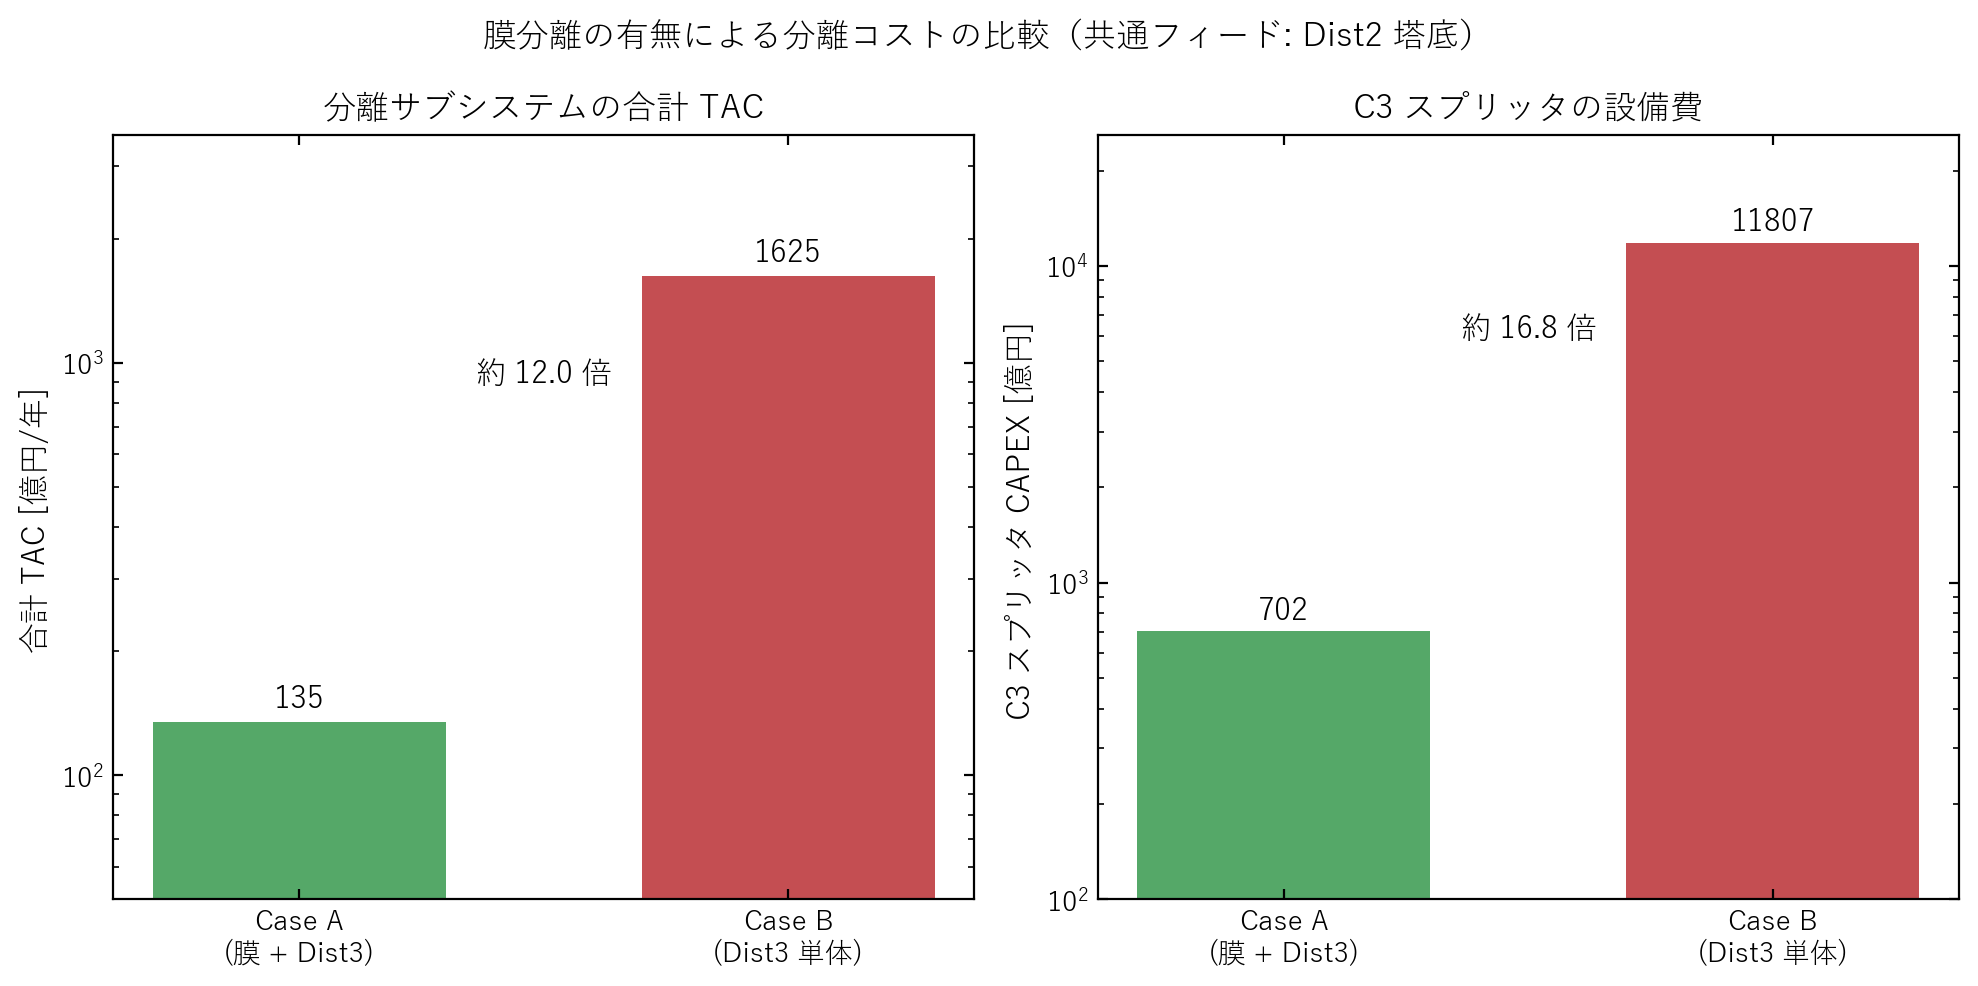
\includegraphics[width=0.82\linewidth]{membrane_vs_dist3}\par
      \vspace{0.15em}
      {\scriptsize 共通フィード $\mathrm{C_3H_6}\,60.7$ mol\%・対数軸}\par
      \vspace{0.3em}
      {\footnotesize\raggedright
        膜なしは合計 TAC が\,{\boldmath\color{SpRed}$12.0$ 倍}\par
        C3 塔設備費が\,{\boldmath\color{SpRed}$16.8$ 倍}に膨らむ\par
        \quad $\to$ 膜の追加投資を大きく上回る削減\par}
    \end{column}

    % ===== 右：採用ハイブリッド構成＋諸元 =========================
    \begin{column}{0.5\textwidth}
      {\bfseries 採用構成　膜 $\to$ C3 スプリッタ}\par
      \vspace{0.2em}
      \centering
      \begin{tikzpicture}[
        >=Stealth, font=\scriptsize,
        u/.style={draw=HeaderBlue, fill=HiBlue!40, rounded corners=2pt,
                  align=center, inner sep=3pt, font=\scriptsize\bfseries,
                  minimum height=8mm},
        io/.style={align=center, font=\scriptsize},
        a/.style={-{Stealth[length=1.8mm]}, line width=0.9pt, rounded corners=2pt},
        rec/.style={-{Stealth[length=1.6mm]}, line width=0.6pt, black!65, rounded corners=2pt},
      ]
        \node[io] (in)  at (0,0)   {塔底 $\mathrm{C_3}$\\{\scriptsize $\mathrm{C_3H_6}\,61$\%}};
        \node[u]  (mem) at (1.9,0) {膜\\分離器};
        \node[u]  (col) at (3.8,0) {C3\\スプリッタ};
        \node[io] (out) at (3.8,1.45) {$\mathrm{C_3H_6}$ 製品\\{\scriptsize $99.5$ wt\%}};
        \draw[a] (in) -- (mem);
        \draw[a] (mem) -- node[above,font=\tiny]{透過 $98.6$\%}(col);
        \draw[a] (col.north) -- (out.south);
        % リサイクル（膜非透過・塔底）
        \draw[rec] (mem.south) |- (1.0,-1.1);
        \draw[rec] (col.south) |- (1.0,-1.1);
        \node[io, anchor=north] at (2.4,-1.05) {$\mathrm{C_3H_8}$ リサイクル};
      \end{tikzpicture}\par
      \vspace{0.3em}
      {\setlength{\fboxsep}{5pt}\setlength{\fboxrule}{1pt}%
       \fcolorbox{HeaderBlue}{white}{%
        \footnotesize\renewcommand{\arraystretch}{1.1}%
        \begin{tabular}{@{}l@{\hspace{1em}}l@{}}
          膜材料        & $\mathrm{ZIF\text{-}8}$ 混合マトリックス膜 \\
          膜選択性 $\alpha$ & $90$　{\scriptsize 蒸留の約 $65$ 倍効率} \\
          総膜面積      & $1.28\times10^{5}\ \mathrm{m^2}$・$256$ 本 \\
          供給圧 $P_H$  & $8.4$ bar・ステージカット $25$\% \\
          C3 塔         & $16.7$ bar・$117$ 段・塔高 $94$ m \\
          製品          & $\mathrm{C_3H_6}\,99.5$ wt\%・$402$ kt/年 \\
        \end{tabular}}}
    \end{column}
  \end{columns}

  \vspace{0.1em}
  \raggedright
  {\footnotesize 膜は蒸留の約 $65$ 倍効率で、\textbf{難所を膜が・仕上げを蒸留が分担}する。}

\end{frame}

\section{水素分離}% =====================================================================
%  12  水素回収 — PSA で副生水素を高純度回収し価値化（型G＋方式選定）
%  source_memo: 08_hydrogen_separation.tex（深冷/膜/PSA比較→PSA採用、活性炭・
%   多成分Langmuir・LDF、吸着↔脱着スイング）＋検証出力。
%   2基(1並列×2)・D4.49m・L24.75m・t_abs742s・t_des113s・β0.254、
%   H2回収率~84%・H2純度99.9%超・CH4捕捉100%、入口1486→H2製品746+オフガス740。
%  方針：左=スイング吸着の模式図＋入出力、右=方式選定＋諸元＋価値化。丸括弧禁止。
% =====================================================================
\begin{frame}

  {\bfseries\large 副生水素を PSA で高純度回収し製品化、残ガスは燃料}\par
  \vspace{0.15em}
  {\footnotesize 脱エタン塔塔頂の $\mathrm{H_2}$ リッチガスを活性炭に通し、$\mathrm{CH_4}\cdot\mathrm{C_2}$ を吸着して非吸着の $\mathrm{H_2}$ を取り出す。}\par

  \vspace{0.5em}

  \begin{columns}[T,onlytextwidth]
    % ===== 左：スイング吸着の模式図＋入出力 =======================
    \begin{column}{0.5\textwidth}
      \centering
      \begin{tikzpicture}[
        >=Stealth, font=\scriptsize,
        bed/.style={draw, minimum width=14mm, minimum height=20mm, align=center,
                    font=\footnotesize\bfseries},
        io/.style={align=center, font=\scriptsize},
        a/.style={-{Stealth[length=1.8mm]}, line width=0.9pt, rounded corners=2pt},
        sw/.style={{Stealth[length=1.6mm]}-{Stealth[length=1.6mm]}, line width=0.6pt, black!60},
      ]
        \node[bed, draw=HeaderBlue, fill=HiBlue!50, text=HeaderBlue] (b1) at (0,0) {吸着};
        \node[bed, pattern=north east lines, pattern color=black!28] (b2) at (3.0,0) {};
        \node[font=\footnotesize\bfseries, align=center] at (b2) {脱着\\再生};
        % 入口フィード（下から吸着塔へ）
        \node[io] (feed) at (0,-2.05) {脱エタン塔塔頂\\$1486$ kmol/h\\{\scriptsize $\mathrm{H_2}\,60$\%}};
        \draw[a] (feed.north) -- (b1.south);
        % H2 製品（吸着塔の上）
        \node[io] (h2) at (0,2.1) {$\mathrm{H_2}$ 製品\\$746$ kmol/h\\{\scriptsize $99.9$\% 超}};
        \draw[a] (b1.north) -- (h2.south);
        % オフガス（脱着塔の下）
        \node[io] (off) at (3.0,-2.05) {オフガス\\$740$ kmol/h\\{\scriptsize 燃料}};
        \draw[a] (b2.south) -- (off.north);
        % スイング
        \draw[sw] (b1.east) -- node[above,font=\tiny]{スイング}(b2.west);
      \end{tikzpicture}\par
      \vspace{0.3em}
      {\scriptsize 常時 $1$ 基吸着・$1$ 基再生の $2$ 基構成で連続供給}
    \end{column}

    % ===== 右：方式選定＋諸元＋価値化 =============================
    \begin{column}{0.5\textwidth}
      {\bfseries 方式選定}\par
      \vspace{0.15em}
      {\footnotesize\raggedright
        深冷分離は $-170\,^\circ$C 級で高コスト、膜は高純度に多段を要す\par
        $\to$\,\textbf{高純度 $99.9$\% 超と工業実績から PSA を採用}\par}

      \vspace{0.4em}
      {\bfseries キー諸元と性能}\par
      \vspace{0.2em}
      {\setlength{\fboxsep}{5pt}\setlength{\fboxrule}{1pt}%
       \fcolorbox{HeaderBlue}{white}{%
        \footnotesize\renewcommand{\arraystretch}{1.1}%
        \begin{tabular}{@{}l@{\hspace{1em}}l@{}}
          吸着材        & 活性炭　{\scriptsize $\mathrm{H_2}$ 非吸着} \\
          総塔数        & $2$ 基　{\scriptsize $1$ 並列 $\times\,2$} \\
          塔径／層高    & $4.49$ m／$24.8$ m \\
          吸着／脱着時間 & $742$ s／$113$ s \\
          $\mathrm{H_2}$ 回収率 & $\approx 84$\% \\
          $\mathrm{H_2}$ 純度   & {\boldmath$99.9$}\% 超・$\mathrm{CH_4}$ 捕捉 $100$\% \\
        \end{tabular}}}

      \vspace{0.4em}
      {\footnotesize\raggedright
        $\mathrm{H_2}$ は製品として販売\par
        オフガスは\textbf{予熱炉の燃料}に充てる\par}
    \end{column}
  \end{columns}

\end{frame}

\end{document}
